\section{WS 1.1 - 18 - MAT - BIP 2018 - OA - Matura 2019/20 1. HT}

\begin{beispiel}[WS 1.1]{1}
Im Jahr 2018 betrug das Bruttoinlandsprodukt (BIP) von Österreich rund 385,71 Milliarden Euro.\\
\begin{tiny}Datenquelle: https://de.statista.com/statistik/daten/studie/14390/umfrage/bruttoinlandsprodukt-in-oesterreich/ [21.11.2019].\end{tiny}

Übersteigen die Einnahmen aus Exporten die Ausgaben aus Importen, so spricht man von einem Leistungsbilanzüberschuss, andernfalls von einem Leistungsbilanzdefizit. In der nachstehenden Abbildung sind für einige Länder diese Überschüsse bzw. Defizite als Leistungsbilanzsalden in Prozent des jeweiligen BIP für das Jahr 2018 angeführt.

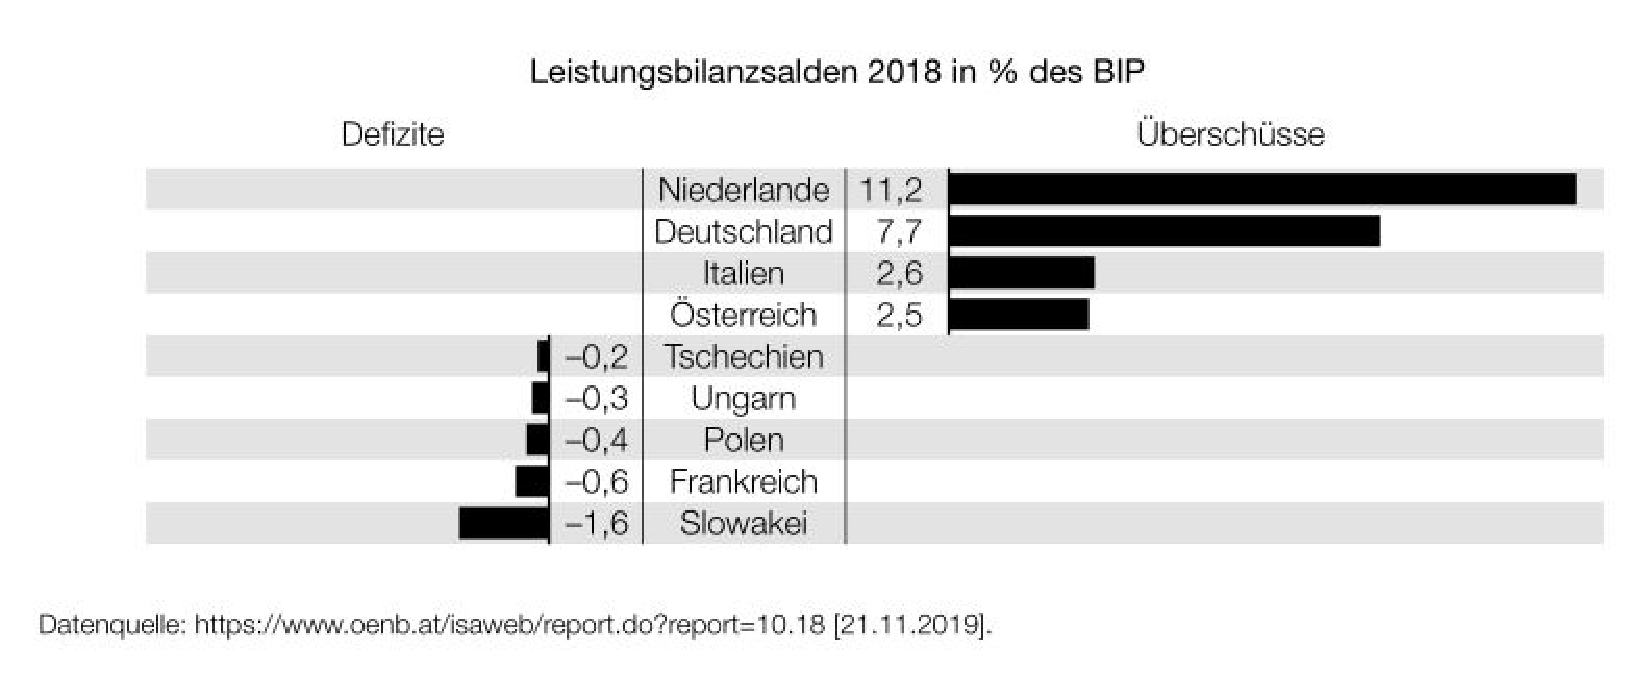
\includegraphics[width=0.9\textwidth]{../_database/Bilder/WS11_18_bip.eps}

Berechne den Leistungsbilanzüberschuss (in Milliarden Euro) von Österreich im Jahr 2018.

Leistungsbilanzüberschuss:\,\,\antwort[\rule{5cm}{0.3pt}]{9,64}\,\, Milliarden Euro
\end{beispiel}